\section{Решение задачи при первом типе ограничений на управление}

В данном пункте рассмотрим ограничения на значения управляющих параметров вида
$$
        v(t) \in \Omega = \{\,[v_1,\,v_2]^\T\in\R^2\;:\;v_1\geqslant 0,\,v_2 \in [m_1,\,m_2]\,\}.
$$
В этом случае задача минимизации равносильна задаче
$$
        J(u) = \int\limits_0^T \left( v_1(t) + \frac{\alpha}{2}\right)^2\,dt \rightarrow \min\limits_{v},\;\mbox{где $v(t) \in \Omega$, $t\in[0,\,T]$,}
$$
при этом задача максимизации функции Гамильтона--Понтрягина эквивалентна максимизации по $v$ следующих выражений:
$$
        \begin{aligned}
        \psi_0\left(v_1+\frac{\alpha}{2}\right) + \psi_2(v_1 - v_2x_2) &\rightarrow \max\limits_{v_1\in [0,\,+\infty)},\\
        -\psi_2x_2v_2&\rightarrow \max\limits_{v_2\in[m_1,\,m_2]}.
        \end{aligned}
$$
Эти задачи имеют следующие решения:
\begin{equation}\label{eq:firstlim_u_1}
        v_1 = 
        \begin{cases}
                \psi_2 - \frac{\alpha}{2}, &\mbox{при $\psi_2 \geqslant \frac{\alpha}{2}$} \\
                0, & \mbox{при $\psi_2 < \frac{\alpha}{2}$},
        \end{cases}
\end{equation}
\begin{equation}\label{eq:firstlim_u_2}
        v_2 = 
        \begin{cases}
                m_2, &\mbox{при $\psi_2x_2<0$} \\
                [m_1,\,m_2], & \mbox{при $\psi_2x_2 = 0$} \\
                m_1, & \mbox{при $\psi_2x_2 > 0$}.
        \end{cases}
\end{equation}

\subsection{Размышления об особом режиме}

Назовём \textit{особым режимом} ситуацию, при которой управление $v$ не определено однозначно. Для задачи \eqref{eq:main_equation} особый режим наступает, когда $\psi_2(t)x_2(t) = 0$\footnote{Условие особого режима}. Рассмотрим при каких условиях особый режим может длиться сколь угодно длительное время, то есть на отрезке $t_0 \leqslant t \leqslant t_1$.
\begin{remark}
        Нам важно рассмотреть эти случаи хотя бы потому, что в начальный момент времени $t = 0$ \textit{тележка} находится в особом режиме.
\end{remark}

На отрезке $t_0 \leqslant t \leqslant t_1$ должно выполняться $\frac{d}{dt} x_2(t)\psi_2(t) = 0$\footnote{Условие удержания в особом режиме}:
$$
        \frac{d}{dt}x_2(t)\psi_2(t) = \dot x_2 \psi_2 + x_2 \dot \psi_2 = (v_1 - v_2x_2)\psi_2 + (-\psi_1^0 + v_2\psi_2)x_2 = 0
$$
$$
        v_1(t)\psi_2(t) = \psi_1^0x_2(t).
$$
Пользуясь последним соотношением, условием особого режима и формулой \eqref{eq:x_2}, получаем, что особый режим будет иметь место и, более того, продолжаться, пока $x_2 = 0$ и $\psi_2(t) < \frac{\alpha}{2}$. Плюс ко всему в особом режиме $v_1(t) \equiv 0$.

Теперь, когда мы знаем значение первой компоненты управления $v_1$ в особом режиме, мы можем получить ещё одно соотношение:
$$
        x_2(t) = -\frac{1}{\psi_2(t)} \Longrightarrow \dot x_2(t) = \frac{\dot\psi_2(t)}{(\psi_2(t))^2},
$$
$$
        \frac{v_2}{\psi_2} = \frac{-\psi_1^0 + v_2\psi_2}{(\psi_2)^2} \Rightarrow \psi_2(t) \equiv -\psi_1^0.      
$$

Как интерпретировать полученные результаты для интересующего нас начального момента времени $t = 0$?
Мы получили альтернативу: в случае, если $\psi_2^0 = \psi_2(0) \geqslant \frac{\alpha}{2}$, \textit{тележка} мгновенно выйдет из особого режима; в случае же, когда $\psi_2^0 = \psi_2(0) < \frac{\alpha}{2}$, \textit{тележка} никогда не сможет покинуть особый режим.

\begin{remark}
        Из-за того, что в особом режиме $v_1(t) \equiv 0$, а $x_2^0 = x_2(0) = 0$ согласно формуле \eqref{eq:x_2} \textit{тележка} будет стоять на месте при начальном выборе $\psi_2^0 < \frac{\alpha}{2}$. Таким управлением нельзя привести \textit{тележку} в конечное состояние $x_1^{\mbox{\textit{кон.}}} = x_1(T) = L > 0$. Поэтому в дальнейшем можем рассматривать только выбор $\psi_2^0 \geqslant \frac{\alpha}{2}$.
\end{remark}

\subsection{Прочие режимы управления}

Расправившись с особым режимом, мы получили также значение управления в сколь угодно малой окрестности нуля: $v_1(t) = \psi_2(t) - \frac{\alpha}{2}$, $v_2(t) = m_1$. Отсутствие длительного особого режима позволяет нам продлить эти управления в начальный момент времени $t=0$ по непрерывности.\footnote{Действительно, значение управления в одной точке роли не играет, так как его вклад в решение производится из интеграла.} В этой же окрестности поведение системы \eqref{eq:auxiliary_system} однозначно определяется фомулой (\ref{eq:psi_2}), которую, взимая интегралы можно переписать в следующем виде:
\begin{equation} \label{eq:firstlim_psi2}
        \psi_2(t) = \underbrace{\left(\psi_2^0 - \frac{\psi_1^0}{m_1}\right)}_Ae^{m_1t} + \underbrace{\frac{\psi_1^0}{m_1}}_B.
\end{equation}
При этом видно, что задание $A$ и $B$ однозначно определяет вид возможной траектории, \textit{подозреваемой} на оптимальность.

Теперь подставим соотношение \eqref{eq:firstlim_psi2} в формулу \eqref{eq:x_2}, чтобы выписать выражения для $x_2(t)$ и $x_1(t)$:
\begin{equation}\label{firstlim_x2}
        x_2(t) = \frac{1}{m_1} \left( A \sh(m_1 t) + \left( B - \frac{\alpha}{2}\right)\left( 1 - e^{-m_1t}\right)\right),
\end{equation}
\begin{equation}\label{firstlim_x1}
        x_1(t) = \frac{1}{m_1} \left(\frac{A}{m_1} (\ch(m_1t) - 1) + \left( B - \frac{\alpha}{2}\right)\left(t - \frac{1}{m_1}\left( 1 - e^{-m_1 t}\right)\right)\right).
\end{equation}
Формулы (\ref{firstlim_x2}) и (\ref{firstlim_x1}) верны, пока $u_1(t) \neq 0$ (то есть пока не наступило \textit{выключение} $u_1$ в момент $\psi_2(t) = \frac{\alpha}{2}$); формула же (\ref{eq:firstlim_psi2}) верна, пока не наступила неопределенность по $u_2$, то есть пока $\psi_2(t) > 0$. 

При этом, если $A > 0$, то $\psi_2(t)$ строго возрастает, и формулы верны при любом $t$. Если же $A < 0$, то формулы (\ref{eq:firstlim_u_1}) и (\ref{eq:firstlim_u_2}) показывают, что нас будут интересовать моменты времени $t_1$ и $t_2$, в которые $\psi_2(t_1) = \frac{\alpha}{2}$ и $\psi_2(t_2) = 0$. В силу строгой монотонности $\psi_2(t)$ эти моменты единственны и $t_1 \leqslant t_2$ ($t_1$ и $t_2$ равны только в ситуации, когда параметр $\alpha$ равен нулю). В дальнейшем будем обозначать $x_j^i = x_j(t_i),\; j=1,\,2,\;i=1,\,2$.

Всвязи с написанным введем следующую классификацию рассматриваемых управлений (и отвечающих им траекторий):
\begin{enumerate}
        \item Пусть $A \geqslant 0$. Тогда будем говорить, что управление реализует \textit{режим акселерации}.
        \item Пусть $A < 0$.
        \begin{enumerate}
                \item Если $t_1 > T$, то будем говорить, что управление реализует \textit{режим отсутствия торможения}.
                \item Если $t_1 < T, \; t_2 > T$, то будем говорить, что управление реализует \textit{режим слабого торможения}.
                \item Если $t_2 < T$, то будем говорить, что управление реализует \textit{режим сильного торможения}.
        \end{enumerate}
\end{enumerate}

\begin{remark}
        Понятно, что при $\alpha = 0$ произойдёт только одно переключение. Мы рассмотрим эту ситуацию отдельно в рассказе о режиме слабого торможения.
\end{remark}

Разберем по порядку каждый из этих режимов. Будем полагать, что оптимальное управление лежит в соответствующем режиме и что для оптимальной траектории $x_2(T) = \xi$ такое, что $S - \varepsilon \leqslant \xi \leqslant S + \varepsilon$.

\subsection{Режимы акселерации и отсутствия торможения}

\begin{figure}[h]
        \hfill
        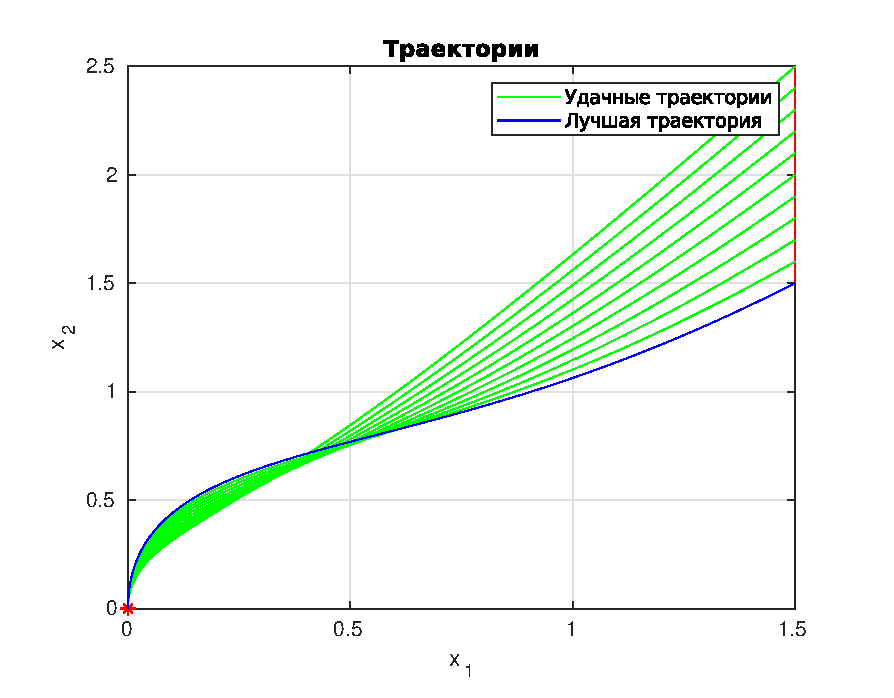
\includegraphics[width=70mm]{first/acc1.eps}
        \hfill
        \hfill
        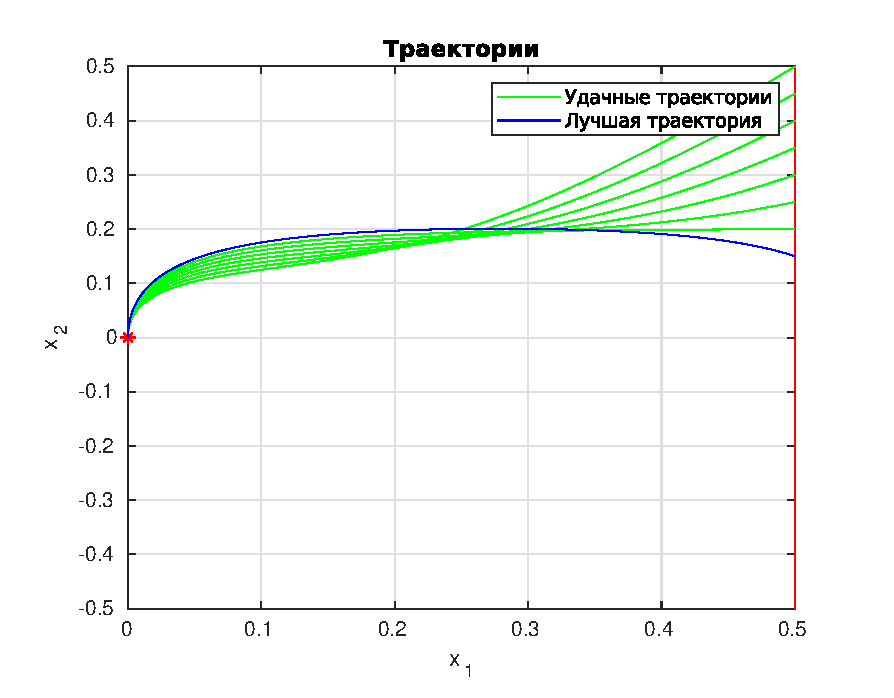
\includegraphics[width=70mm]{first/acc2.eps}
        \hfill
        \caption{Перебираемые траектории в режимах акселерации и отсутствия торможения для двух разных постановок задач. Слева присутствуют только траектории в режиме аксерерации. Справа же присутствуют и траектории в режиме отсутствия торможения (более того, одна из них оказалась лучшей).}
\end{figure}

Как уже было отмечено, в этом случае поведение системы описывается уравнениями (\ref{eq:firstlim_psi2}), (\ref{firstlim_x2}) и (\ref{firstlim_x1}).

Из (\ref{eq:firstlim_psi2}) и (\ref{firstlim_x2}) следует, что соотношения $x_1(T) = L$ и $x_2(T) = \xi$ являются линейной системой относитльно $A$ и $B$. После этого, если $A < 0$, то необходимо проверить условия:
$$
\psi_2^0 = A + B \geqslant \frac{\alpha}{2} \qquad \mbox{и} \qquad t_1 > T \Leftrightarrow \frac{1}{m_1} \ln \frac{\frac{\alpha}{2} - B}{A} > T,
$$
чтобы проверить, действительно ли реализуется режим отсутствия торможения. Зная $A$ и $B$, мы получим $\psi_1^0$ и $\psi_2^0$, что позволяет полностью восстановить управление и траекторию.

%%%%%%%%%%%%%%%%%%%%%%%%%%%%%%%%%%%%%%
%                                    %
%          Слабое торможение         %
%                                    %
%%%%%%%%%%%%%%%%%%%%%%%%%%%%%%%%%%%%%%
\subsection{Режим слабого торможения}

\begin{figure}[h]
        \hfill
        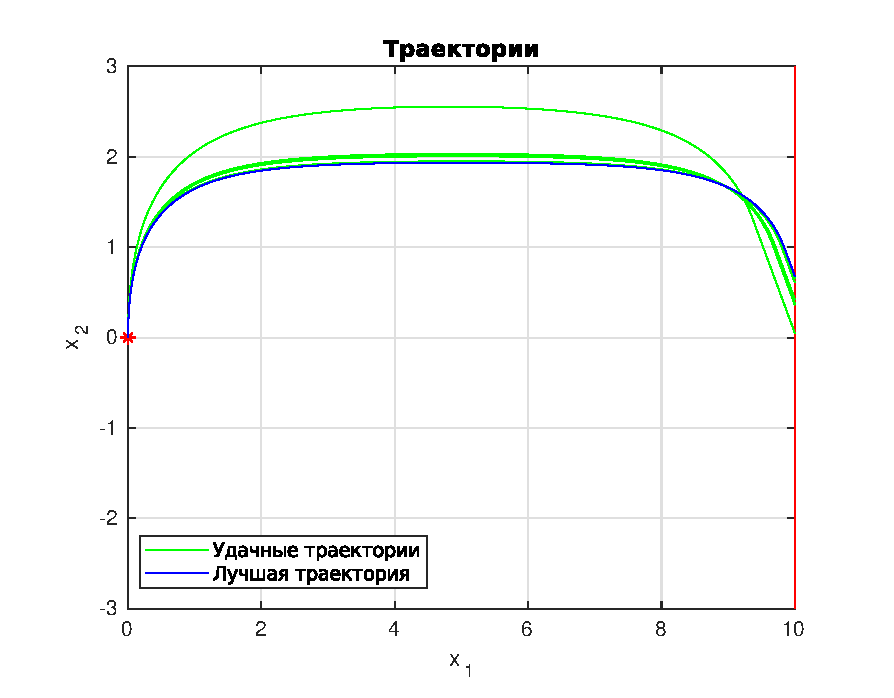
\includegraphics[width=70mm]{first/weak1.eps}
        \hfill
        \hfill
        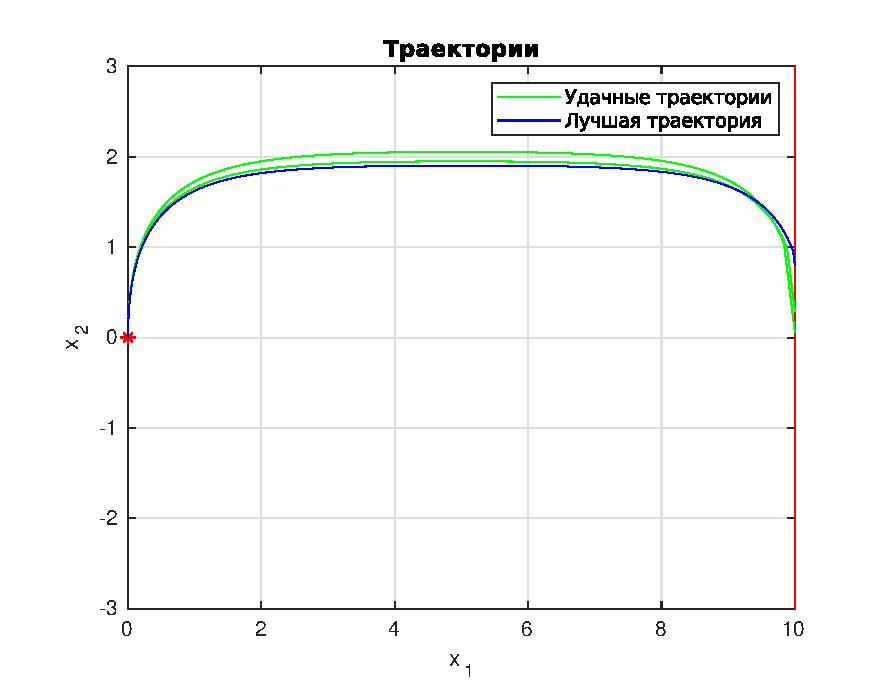
\includegraphics[width=70mm]{first/weak2.eps}
        \hfill
        \caption{Перебираемые траектории в режиме слабого торможения. Слева для $\alpha = 1 > 0$, справа для той же задачи при $\alpha = 0$.}
\end{figure}

\subsubsection{Задача с параметром $\alpha > 0$}
От момента времени $t_1$ до момента $T$ система будет описываться уравнениями:
\begin{equation} \label{eq:firslim_weak_x2}
        x_2(t) = x_2^1e^{m_1(t_1 - t)},
\end{equation}
\begin{equation} \label{eq:firslim_weak_x1}
        x_1(t) = x_1^1 + \frac{x_2^1}{m_1}+\left(1 - e^{m_1(t_1 - t)}\right).
\end{equation}

Устроим перебор по времени переключения $0 < t_1 < T$ и конечной точки траектории $S-\varepsilon \leqslant \xi \leqslant S + \varepsilon$. Соотношение $x_2(T) = \xi$ дает
$$
        x_2^1 = \xi e^{m_1(T - t_1)},
$$
из соотношения $x_1(T) = L$ же получается
$$
        x_1^1 = L - \frac{x_2^1 - \xi}{m_1}.
$$

Далее можно поступить аналогично случаю отсутствия торможения. Кроме того необходимо проверить условия реализации этого режима:
$$
        A < 0, \quad \psi_2^0 = A + B > \frac{\alpha}{2}, \quad t_2 = \frac{1}{m_1}\ln\left(-\frac{B}{A}\right) > T \quad \mbox{и} \quad \psi_2(t_1) = A e^{m_1t_1} + B = 0.
$$

\subsubsection{Задача с параметром $\alpha = 0$}

Данный случай является полностью аналогичным рассмотренному ранее, с единственным отличием: теперь траектории на отрезке $t_1 \leqslant t \leqslant T$ будут определяться следующими соотношениями:
$$
        x_1(t) = x_1^1 + \frac{x_2^1}{m_2}+\left(1 - e^{m_2(t_1 - t)}\right), \qquad
        x_2(t) = x_2^1e^{m_2(t_1 - t)}.
$$

Кроме того, при нулевом значении параметра $\alpha$ дальнейшие переключения невозможны, а, значит, дальнейшие режимы рассматривать не нужно.


%%%%%%%%%%%%%%%%%%%%%%%%%%%%%%%%%%%%%
%%%%%%%%%%%%%%%%%%%%%%%%%%%%%%%%%%%%%
%%%%%%%%%%%%%%%%%%%%%%%%%%%%%%%%%%%%%
%%%%%%%%%%%%%%%%%%%%%%%%%%%%%%%%%%%%%
%%%%%%%%%%%%%%%%%%%%%%%%%%%%%%%%%%%%%

\subsection{Режим сильного торможения}
\begin{figure}[h]
        \hfill
        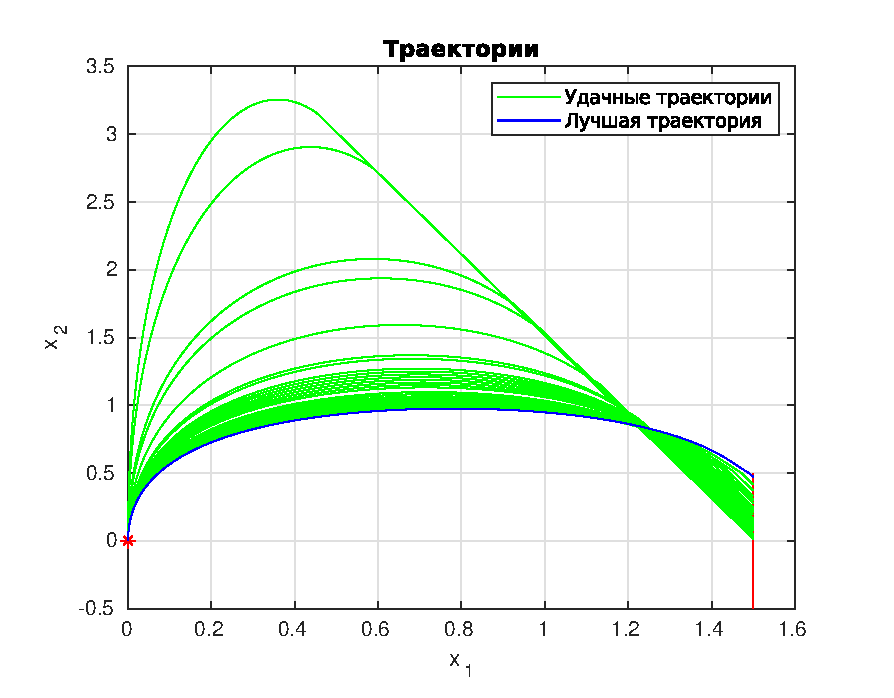
\includegraphics[width=70mm]{first/strong1.eps}
        \hfill
        \hfill
        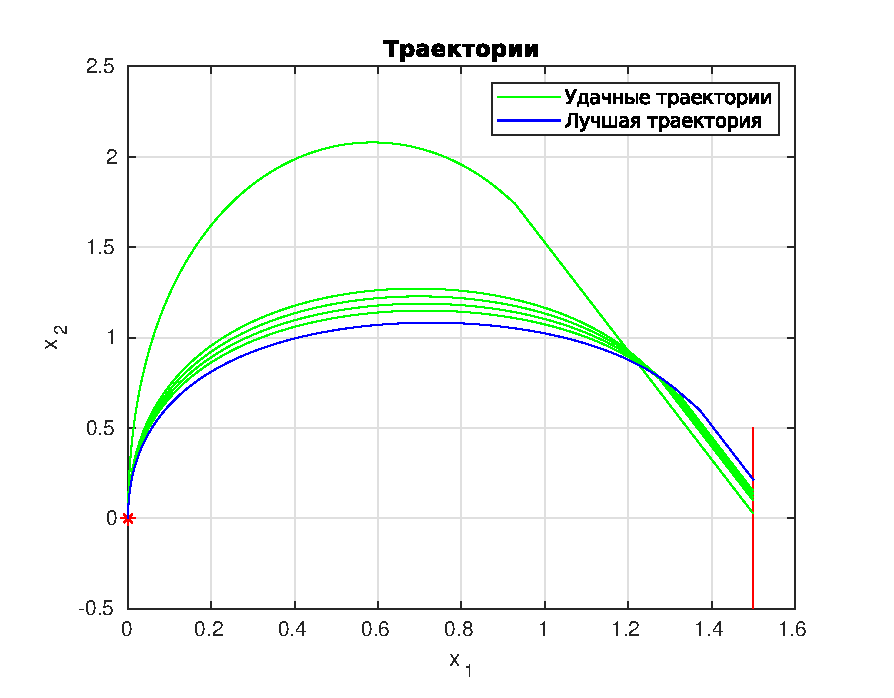
\includegraphics[width=70mm]{first/strong2.eps}
        \hfill
        \caption{Перебираемые траектории в режиме сильного торможения. Представлены траектории для одной задачи при разном числе разбиения. Отрезок $0 \leqslant t \leqslant T$ был разбит на 1000 частей слева и на 500 частей справа.}
\end{figure}
В этом режиме соотношения (\ref{eq:firslim_weak_x2}) и (\ref{eq:firslim_weak_x1}) определяют поведение системы на отрезке $t_1 \leqslant t \leqslant t_2$, а на отрезке $t_2 \leqslant t \leqslant T$ ее буду описывать следующие соотношения
\begin{equation}\label{eq:strong}
        x_1(t) =x_1^2 + \frac{x_2^2}{m_2}\left(1 - e^{m_2(t_2-t)}\right),
        \qquad
        x_2(t) = x_2^2e^{m_2(t_2-t)}
\end{equation}

Устроим перебор по временам первого и второго переключений $0 < t_1 < T$, $t_1 < t_2 < T$. Так как соотношение \eqref{eq:firstlim_psi2} верно на отрезке $0 \leqslant t \leqslant t_2$, то выражения
$$
        \psi_2(t_1) = Ae^{m_1t_1} + B = \frac{\alpha}{2}
        \quad \mbox{и} \quad
        \psi_2(t_2) = Ae^{m_1t_1} + B = 0
$$
образуют систему линейных алгебраических уравнений относительно неизвестных $A$ и $B$. Зная, эти параметры мы можем восстановить управление и траекторию на всем отрезке $0 \leqslant t \leqslant T$. После чего необходимо проверить траекторию на реализуемость
$$
        A < 0, \qquad \psi_2^0 = A+B \geqslant \frac{\alpha}{2}
$$
и на попадание траектории в целевое множество
$$
        x_1(T) = L, \qquad x_2(T) \in [S-\varepsilon,\, S+\varepsilon].
$$

